\documentclass{article}
\usepackage{helvet}


\usepackage{cite}
\usepackage{amsmath,amssymb,amsfonts}
\usepackage{mathtools, amssymb, bm}
\usepackage{algorithmic}
\usepackage{graphicx}
\usepackage{textcomp}
\usepackage{xcolor}
\usepackage{hyperref}
\usepackage{placeins}
\usepackage{graphicx}
\usepackage{subcaption}
\usepackage[utf8]{inputenc}
\usepackage[DIV=16]{typearea}
\usepackage{microtype}
\usepackage{mathtools, amssymb, bm}
\newcommand{\op}{\operatorname}
\usepackage{parskip}
\usepackage[shortlabels]{enumitem}
\usepackage{graphicx}
\usepackage{subcaption}
\usepackage{listings}



\def\BibTeX{{\rm B\kern-.05em{\sc i\kern-.025em b}\kern-.08em
    T\kern-.1667em\lower.7ex\hbox{E}\kern-.125emX}}


\title{Question 2, Assignment 3: CS 754, Spring 2024-25}
\author{
\IEEEauthorblockN{
    \begin{tabular}{cccc}
        \begin{minipage}[t]{0.23\textwidth}
            \centering
            Amitesh Shekhar\\
            IIT Bombay\\
            22b0014@iitb.ac.in
        \end{minipage} & 
        \begin{minipage}[t]{0.23\textwidth}
            \centering
            Anupam Rawat\\
            IIT Bombay\\
            22b3982@iitb.ac.in
        \end{minipage} & 
        \begin{minipage}[t]{0.23\textwidth}
            \centering
            Toshan Achintya Golla\\
            IIT Bombay\\
            22b2234@iitb.ac.in
        \end{minipage} \\
        \\ 
    \end{tabular}
}
}

\date{March 21, 2025}


\usepackage{amsmath}
\usepackage{amssymb}
\usepackage{hyperref}
\usepackage{ulem,graphicx}
\usepackage[margin=0.5in]{geometry}

\begin{document}
\maketitle

\textbf{Declaration:} The work submitted is our own, and
we have adhered to the principles of academic honesty while completing and submitting this work. We have not
referred to any unauthorized sources, and we have not used generative AI tools for the work submitted here.

\begin{enumerate}
\item In class, we studied a video compressive sensing architecture from the paper `Video from a single exposure coded snapshot' published in ICCV 2011 (See \url{http://www.cs.columbia.edu/CAVE/projects/single_shot_video/}). Such a video camera acquires a `coded snapshot' $E_u$ in a single exposure time interval $u$. This coded snapshot is the superposition of the form $E_u = \sum_{t=1}^T C_t \cdot F_t$ where $F_t$ is the image of the scene at instant $t$ within the interval $u$ and $C_t$ is a randomly generated binary code at that time instant, which modulates $F_t$. Note that $E_u$, $F_t$ and $C_t$ are all 2D arrays. Also, the binary code generation as well as the final summation all occur within the hardware of the camera. Your task here is as follows:
\begin{enumerate}
\item Read the `cars' video in the homework folder in MATLAB using the `mmread' function which has been provided in the homework folder and convert it to grayscale. Extract the first $T = 3$ frames of the video. You may use the following code snippet: \\
\texttt{A = mmread('cars.avi');
T = 3;
for i=1:T,  X(:,:,i) = double(rgb2gray(A.frames(i).cdata)); \ end;
[H,W,T] = size(X);
}
\item Generate a $H \times W \times T$ random code pattern whose elements lie in $\{0,1\}$. Compute a coded snapshot using the formula mentioned and add zero mean Gaussian random noise of standard deviation 2 to it. Display the coded snapshot in your report.
\item Given the coded snapshot and assuming full knowledge of $C_t$ for all $t$ from 1 to $T$, your task is to estimate the original video sequence $F_t$. For this you should rewrite the aforementioned equation in the form $\boldsymbol{Ax} = \boldsymbol{b}$ where $\boldsymbol{x}$ is an unknown vector (vectorized form of the video sequence). Mention clearly what $\boldsymbol{A}$ and $\boldsymbol{b}$ are, in your report.
\item You should perform the reconstruction using either the ISTA algorithm or the OMP algorithm (the original paper used OMP). You can re-use your own code from a previous assignment. For computational efficiency, we will do this reconstruction patchwise. Write an equation of the form $\boldsymbol{Ax} = \boldsymbol{b}$ where $\boldsymbol{x}$ represents the $i$th patch from the video and having size (say) $8 \times 8 \times T$ and mention in your report what $\boldsymbol{A}$ and $\boldsymbol{b}$ stand for. For perform the reconstruction, assume that each $8 \times 8$ slice in the patch is sparse or compressible in the 2D-DCT basis. 
\item Repeat the reconstruction for all overlapping patches and average across the overlapping pixels to yield the final reconstruction. Display the reconstruction and mention the relative mean squared error between reconstructed and original data, in your report as well as in the code. 
\item Repeat this exercise for $T = 5, T = 7$ and mention the mention the relative mean squared error between reconstructed and original data again.
\item \textbf{Note: To save time, extract a portion of about $120 \times 240$ around the lowermost car in the cars video and work entirely with it. In fact, you can show all your results just on this part. Some sample results are included in the homework folder.}
\item Repeat the experiment with any consecutive 5 frames of the `flame' video from the homework folder. 
\textsf{[20 points = 12 points for correct implementation + 4 points for correct expressions for $A$,$b$; 4 points for display results correctly.]}
\end{enumerate}
\\
    \makebox[0pt][l]{\hspace{-7pt}\textit{Soln:}} % Aligns "Answer:" to the left

\newpage

\section{Theory}

We know that the final 2-D image $I(x,y)$ is given by
\begin{equation}{\label{eq:hitomi}}
I(x,y) = \sum_{t=1}^T C_t(x,y)\cdot F_t(x,y)\ \forall\ x,y
\end{equation}
We can rewrite the expression in terms of matrix-vector product where each pixel signifies an element of the vector as below
\begin{equation}
\underbrace{
	\begin{bmatrix}
	\op{diag}(\op{vec}(C_1)) & \op{diag}(\op{vec}(C_2)) & \cdots & \op{diag}(\op{vec}(C_T))
	\end{bmatrix}
}_{\bm{A}\in\mathbb{R}^{HW\times HWT}}
\underbrace{
	\begin{bmatrix}
	\op{vec}(F_1) \\ \op{vec}(F_2) \\ \vdots \\ \op{vec}(F_T)
	\end{bmatrix}
}_{\bm{x}\in\mathbb{R}^{HWT}}
=
\underbrace{
	\begin{bmatrix}
	\op{vec}(I)
	\end{bmatrix}
}_{\bm{b}\in\mathbb{R}^{HW}}
\end{equation}
Here, $\op{vec}(\bm{A})$ is conversion of an $m\times n$ matrix into a $mn-$sized vector. 


Moreover, for each patch $i$, we can write $\bm{A}=\bm{\Phi}\bm{\Psi}$, where $\bm{\Phi}$ is the measurement matrix and $\bm{\Psi}$ is the sparsifying basis matrix (common for all patches). Now, for each time frame $F_i$, we can write $\bm{H}\in\mathbb{R}^{H_pW_p\times H_pW_p}$ such that $\op{vec}(F_t) = \bm{H}\op{vec}(\hat{F}_t)$ where $\bm{H}$ is taken as the 2-D DCT matrix.
\begin{equation}
\underbrace{
	\overbrace{
		\begin{bmatrix}
			\op{diag}(\op{vec}(C_1)) & \op{diag}(\op{vec}(C_2)) & \cdots & \op{diag}(\op{vec}(C_T))
		\end{bmatrix}
	}^{\bm{\Phi}\in\mathbb{R}^{H_pW_p\times H_pW_pT}}
	\overbrace{
		\begin{bmatrix}
			\bm{H} & \bm{0} & \cdots & \bm{0}\\
			\bm{0} & \bm{H} & \cdots & \bm{0}\\
			\vdots & \vdots & \ddots & \vdots\\
			\bm{0} & \bm{0} & \cdots & \bm{H}\\
		\end{bmatrix}
	}^{\bm{\Psi}\in\mathbb{R}^{H_pW_pT\times H_pW_pT}}
}_{\bm{A}}
\underbrace{
	\begin{bmatrix}
	\op{vec}(\hat{F}_1) \\ \op{vec}(\hat{F}_2) \\ \vdots \\ \op{vec}(\hat{F}_T)
	\end{bmatrix}
}_{\bm{\theta}\in\mathbb{R}^{H_pW_pT}}
=
\underbrace{
	\begin{bmatrix}
	\op{vec}(I)
	\end{bmatrix}
}_{\bm{b}\in\mathbb{R}^{H_pW_p}}
\end{equation}
Here, the dimensions of each patch is $(H_p, W_p)=(8,8)$. \newline


Above part contained the theory required for the question. ISTA algorithm was used for reconstruction purposes. The full code for running the required algorithm(s) is present in the \hyperlink{../code/code.m}{code} file.\\
Attaching the results obtained from running the code:
\section{Results}

\subsection{Coded Snapshots}

\begin{figure}[h!]
    \centering
    \begin{subfigure}{0.3\textwidth}
        \centering
        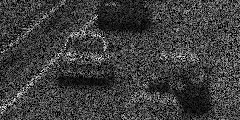
\includegraphics[width=\linewidth]{../images/cars/coded snapshot, T = 3.png}
        \caption{Coded Snapshot, T = 3 (Cars)}
    \end{subfigure}
    \begin{subfigure}{0.3\textwidth}
        \centering
        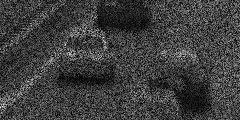
\includegraphics[width=\linewidth]{../images/cars/coded snapshot, T = 5.png}
        \caption{Coded Snapshot, T = 5 (Cars)}
    \end{subfigure}
    \begin{subfigure}{0.3\textwidth}
        \centering
        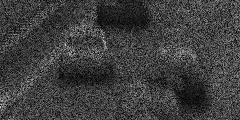
\includegraphics[width=\linewidth]{../images/cars/coded snapshot, T = 7.png}
        \caption{Coded Snapshot, T = 7 (Cars)}
    \end{subfigure}
    \begin{subfigure}{0.3\textwidth}
        \centering
        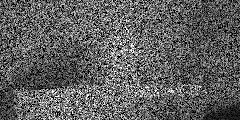
\includegraphics[width=\linewidth]{../images/flame/coded snapshot, T = 3.png}
        \caption{Coded Snapshot, T = 3 (Flame)}
    \end{subfigure}
    \begin{subfigure}{0.3\textwidth}
        \centering
        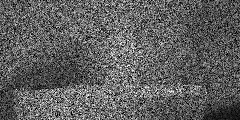
\includegraphics[width=\linewidth]{../images/flame/coded snapshot, T = 5.png}
        \caption{Coded Snapshot, T = 5 (Flame)}
    \end{subfigure}
    \begin{subfigure}{0.3\textwidth}
        \centering
        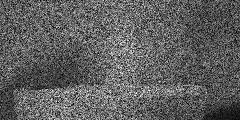
\includegraphics[width=\linewidth]{../images/flame/coded snapshot, T = 7.png}
        \caption{Coded Snapshot, T = 7 (Flame)}
    \end{subfigure}
    \caption{Coded Snapshots for Cars and Flame Videos at Different T Values}
\end{figure}

\newpage

\subsection{Frame Sequences}
\begin{figure}[h!]
    \centering
    % Row 1: 4 frames
    \begin{subfigure}{0.24\textwidth}
        \centering
        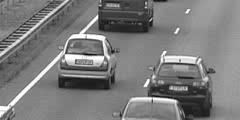
\includegraphics[width=\linewidth]{../images/cars/frame = 1.png}
        \caption{Frame 1}
    \end{subfigure}
    \begin{subfigure}{0.24\textwidth}
        \centering
        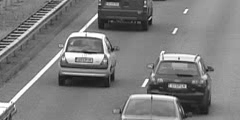
\includegraphics[width=\linewidth]{../images/cars/frame = 2.png}
        \caption{Frame 2}
    \end{subfigure}
    \begin{subfigure}{0.24\textwidth}
        \centering
        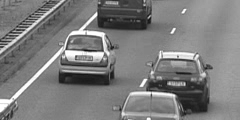
\includegraphics[width=\linewidth]{../images/cars/frame = 3.png}
        \caption{Frame 3}
    \end{subfigure}
    \begin{subfigure}{0.24\textwidth}
        \centering
        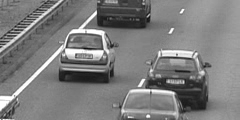
\includegraphics[width=\linewidth]{../images/cars/frame = 4.png}
        \caption{Frame 4}
    \end{subfigure}

    % Row 2: 3 frames
    \vskip 0.2cm
    \begin{subfigure}{0.32\textwidth}
        \centering
        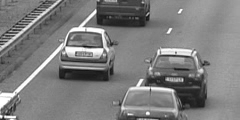
\includegraphics[width=\linewidth]{../images/cars/frame = 5.png}
        \caption{Frame 5}
    \end{subfigure}
    \begin{subfigure}{0.32\textwidth}
        \centering
        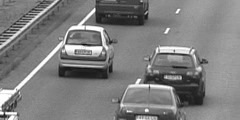
\includegraphics[width=\linewidth]{../images/cars/frame = 6.png}
        \caption{Frame 6}
    \end{subfigure}
    \begin{subfigure}{0.32\textwidth}
        \centering
        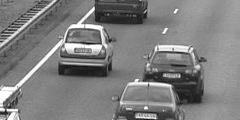
\includegraphics[width=\linewidth]{../images/cars/frame = 7.png}
        \caption{Frame 7}
    \end{subfigure}

    \caption{Extracted frames from the Cars video}
    \label{fig:cars_frames}
\end{figure}


\begin{figure}[h!]
    \centering
    % Row 1: 4 frames
    \begin{subfigure}{0.24\textwidth}
        \centering
        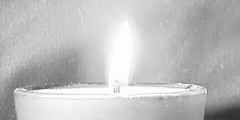
\includegraphics[width=\linewidth]{../images/flame/frame = 1.png}
        \caption{Frame 1}
    \end{subfigure}
    \begin{subfigure}{0.24\textwidth}
        \centering
        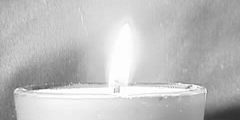
\includegraphics[width=\linewidth]{../images/flame/frame = 2.png}
        \caption{Frame 2}
    \end{subfigure}
    \begin{subfigure}{0.24\textwidth}
        \centering
        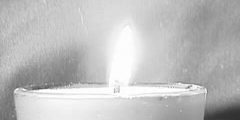
\includegraphics[width=\linewidth]{../images/flame/frame = 3.png}
        \caption{Frame 3}
    \end{subfigure}
    \begin{subfigure}{0.24\textwidth}
        \centering
        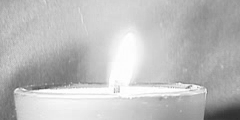
\includegraphics[width=\linewidth]{../images/flame/frame = 4.png}
        \caption{Frame 4}
    \end{subfigure}

    % Row 2: 3 frames
    \vskip 0.2cm
    \begin{subfigure}{0.32\textwidth}
        \centering
        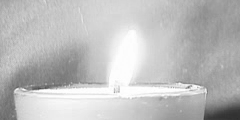
\includegraphics[width=\linewidth]{../images/flame/frame = 5.png}
        \caption{Frame 5}
    \end{subfigure}
    \begin{subfigure}{0.32\textwidth}
        \centering
        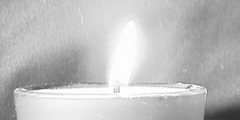
\includegraphics[width=\linewidth]{../images/flame/frame = 6.png}
        \caption{Frame 6}
    \end{subfigure}
    \begin{subfigure}{0.32\textwidth}
        \centering
        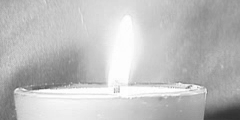
\includegraphics[width=\linewidth]{../images/flame/frame = 7.png}
        \caption{Frame 7}
    \end{subfigure}

    \caption{Extracted frames from the Flame video}
    \label{fig:flame_frames}
\end{figure}
\subsection{Reconstructed Frames}

\begin{figure}[h!]
    \centering
    \begin{subfigure}{0.3\textwidth}
        \centering
        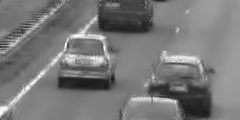
\includegraphics[width=\linewidth]{../images/cars/reconstructed, T = 3, frame = 1.png}
        \caption{Reconstructed, T = 3, Frame = 1 (Cars)}
    \end{subfigure}
    \begin{subfigure}{0.3\textwidth}
        \centering
        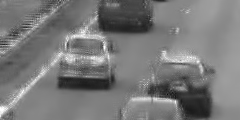
\includegraphics[width=\linewidth]{../images/cars/reconstructed, T = 5, frame = 1.png}
        \caption{Reconstructed, T = 5, Frame = 1 (Cars)}
    \end{subfigure}
    \begin{subfigure}{0.3\textwidth}
        \centering
        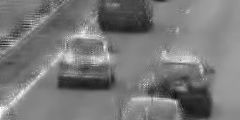
\includegraphics[width=\linewidth]{../images/cars/reconstructed, T = 7, frame = 1.png}
        \caption{Reconstructed, T = 7, Frame = 1 (Cars)}
    \end{subfigure}
    \begin{subfigure}{0.3\textwidth}
        \centering
        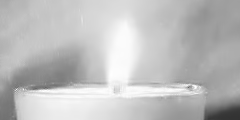
\includegraphics[width=\linewidth]{../images/flame/reconstructed, T = 3, frame = 1.png}
        \caption{Reconstructed, T = 3, Frame = 1 (Flame)}
    \end{subfigure}
    \begin{subfigure}{0.3\textwidth}
        \centering
        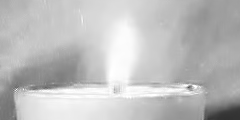
\includegraphics[width=\linewidth]{../images/flame/reconstructed, T = 5, frame = 1.png}
        \caption{Reconstructed, T = 5, Frame = 1 (Flame)}
    \end{subfigure}
    \begin{subfigure}{0.3\textwidth}
        \centering
        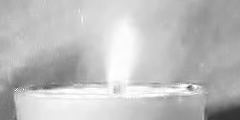
\includegraphics[width=\linewidth]{../images/flame/reconstructed, T = 7, frame = 1.png}
        \caption{Reconstructed, T = 7, Frame = 1 (Flame)}
    \end{subfigure}
    \caption{Reconstructed Frames for Different T Values}
\end{figure}
\newpage 
\subsection{Reconstruction Losses}
\begin{table}[h!]
    \centering
    \caption{Relative Mean Squared Error (RMSE) for Reconstructed Videos}
    \label{tab:rmse_results}
    \begin{tabular}{|l|c|c|c|}
        \hline
        \textbf{Video} & \textbf{T = 3} & \textbf{T = 5} & \textbf{T = 7} \\
        \hline
        Cars  & 0.12107 & 0.14484 & 0.16047 \\
        Flame & 0.025309 & 0.028312 & 0.032038 \\
        \hline
    \end{tabular}
\end{table}

\section{Excerpt from the Code}
\begin{lstlisting}[language=Matlab, caption=Reading and Preprocessing the Video, label=code:read_video]
% Read and preprocess video
video_input = mmread(char("../images/"+ image_name +".avi"));
start_frame = start_frames(image_name);
for i=1:T
    X(:,:,i) = double(rgb2gray(video_input.frames(i+start_frame-1).cdata));
end
% Cropping region of interest
H = dimensions(1);
W = dimensions(2);
X = X(start_heights(image_name):start_heights(image_name)+H-1, ...
      start_widths(image_name):start_widths(image_name)+W-1, :);
\end{lstlisting}

\begin{lstlisting}[language=Matlab, caption=Generating Coded Snapshot, label=code:coded_snapshot]
% Generate coded snapshot
code = randi([0 1], size(X));  % Random binary code
coded_snapshot = X .* code;
coded_snapshot = sum(coded_snapshot, 3) + generate_gaussian_noise(dimensions, 0, 4);
\end{lstlisting}

\begin{lstlisting}[language=Matlab, caption=ISTA Algorithm for Reconstruction, label=code:ista]
function theta = ista(y, A, threshold, lambda)
    theta = randn([size(A,2) 1]); % Random initialization
    alpha = eigs(A'*A,1); % Compute step size
    while true
        theta_next = wthresh(theta + 1/alpha*A'*(y-A*theta), 's', lambda / (2*alpha));
        if norm(theta_next-theta) < threshold
            break;
        end
        theta = theta_next;
    end
end
\end{lstlisting}

\begin{lstlisting}[language=Matlab, caption=Calculating RMSE, label=code:rmse]
function RMSE = calculate_RMSE(image_original, image_reconstructed)
    RMSE = norm(image_reconstructed(:) - image_original(:)) / norm(image_original(:));
end
\end{lstlisting}


\end{enumerate}
\end{document}